% !TEX root = machine_learning.tex





\chapter[Linear Regression]{Linear Models for Regression}
\label{chap:lin.reg}

In  regression, {\em linear models}  refer to situations in which one tries to predict the dependent variable $Y\in \CR_Y = \mR^{q}$ by a function $\hf(X)$ of the dependent variable $X\in \CR_X$, where  $\hf$ is optimized over a {\em linear space} $\CF$. 
The most common situation is the ``standard linear model,'' for which $\CR_X = \mR^d$ and%\,\footnote{We denote by  $\CM_{d,q}(\mR)$ the vector space of all $d$ by $q$ matrices with real entries.}
\begin{equation}
\label{eq:cf.linear}
\CF = \{ f(x) = {a_0} + b^{T}x: {a_0}\in \mR^{q}, b\in \CM_{d,q}(\mR)\}.  
\end{equation}

More generally, with $q=1$, given a mapping $h : \CR \to H$, where $H$ is an inner-product space, one can take:
\begin{equation}
\label{eq:cf.feature}
\CF = \{ f(x) = {a_0} + \scp{b}{h(x)}_{H}: {a_0}\in \mR, b\in H\}.  
\end{equation}
Note that $h$ can be nonlinear, and $\CF$ can be infinite dimensional. Such sets corresponds to linear models using feature functions, and will be addressed using kernel methods in this chapter.

Note also that, even if the model is linear, the associated training algorithms can be nonlinear, and we
will review in fact several situations in which solving the estimation problem requires nonlinear optimization methods. 



\section{Least-Square  Regression}
\subsection{Notation and Basic Estimator}
We denote by $Y$ and $X$ the dependent and independent variables of the regression problem. We will assume that $Y$ takes values in  $\mR^q$ and that $X$ takes values in a set $\CR_X$, which will, by default, be equal to $\mR^d$, except when discussing kernel methods, for which this set can be arbitrary (provided that there is a mapping $h$ from $\CR_X$ to  an inner product space $H$ with an easily computable kernel). 
 
Least-square regression uses the risk function $r(y,y') = |y-y'|^2$. The prediction error is then $R(f) = E(|Y-f(X)|^2)$ for any predictor $f$ and the Bayes predictor is the conditional expectation $x \mapsto E(Y\mid X=x)$ (see \cref{item:Bayes.MSE} in \cref{sec:bayes.pred}). We also start with the standard setting where $\CR_X = \mR^d$ and
$\CF$ given by \eqref{eq:cf.linear}. 

We will use the following notation, which sometimes simplifies the computation. If $x\in \mR^d$, we let $\tilde x = \begin{pmatrix}1\\x\end{pmatrix}$, which belongs to $\mR^{d+1}$. The linear predictor 
$
f(x) = {a_0} + b^T x
$
with ${a_0}\in \mR^{q}, b\in \CM_{d,q}(\mR)$ can then be written as $f(x) = \beta^{T} \tilde x$ with $\beta =
\begin{pmatrix} a_0^{T}\\ b\end{pmatrix} \in \CM_{d+1,q}(\mR)$.  

In a model-based approach, the linear model is a Bayes predictor under the generative assumption that $Y = {a_0} + b^T X + \ep$ where $\ep$ is a residual noise satisfying $E(\ep\mid X) = 0$, which is true, for example, when $\ep$ is centered and independent of $X$. If one further specifies the model so that $\ep$ is Gaussian, centered and independent of $X$, and one  assumes that the distribution of $X$ does not depend on ${a_0}$ and $b$, then the maximum likelihood estimator of these parameters based on a training set $T = ((x_1, y_1), \ldots, (x_N, y_N))$ must minimize the ``residual sum of squares:''
\[
RSS(\be) \defeq N\hat R(f) \defeq \sum_{k=1}^N |y_k - f(x_k)|^2  = \sum_{k=1}^N |y_k -
\be^{T} \tx_k|^2 \,.
\]
In other terms, the model-based approach is identical, under these (standard) assumptions, to empirical risk minimization (\cref{sec:emp.risk}), on which we now focus. (Recall that, even when using a model-based approach, one does not make assumptions on the true distribution of $X$ and $Y$; one rather treats the model as an approximation of these distributions, estimated by maximum likelihood, and uses the Bayes predictor for the estimated model.) 

The computation of the optimal regression parameters is made easier by the introduction of the following matrices.
 Introduce the $N\ti (d+1)$ matrix $\mathcal X$ with rows $\tilde x_1^T, \ldots, \tilde x_N^T$ and the $N\ti q$ matrix 
$\mathcal Y$ with rows $y_1^{T}, \ldots, y_N^{T}$, 
that is:
\[
 \CX = \begin{pmatrix} 1 & \pe{x_1}{1} & \cdots & \pe{x_1}{d} \\ \vdots & \vdots && \vdots \\  1 & \pe{x_N}{1} & \cdots & \pe{x_N}{d} \end{pmatrix}, \quad
 \CY = \begin{pmatrix} \pe{y_1}{1} & \cdots & \pe{y_1}{q} \\ \vdots && \vdots \\  \pe{y_N}{1} & \cdots & \pe{y_N}{q}\end{pmatrix}\,.
\]
With this notation, we have
\[
RSS(\be) = |\mathcal Y - \mathcal X \be|_{2}^2.
\]
with $|A|_{2}^{2} = \trace(A^{T}A)$ for a rectangular matrix $A$. The solution of the problem is then provided by the following theorem.
\begin{theorem}
\label{th:ls.reg}
Assume that the matrix $\mathcal X$ has rank $d+1$. Then the RSS is
minimized for 
\[
\hat \beta = (\CX^T\CX)^{-1} \CX^T \mathcal Y
\]
\end{theorem}
\begin{proof}
We provide two possible proofs of this elementary problem. The first one is an optimization argument noting that
$F(\be) \defeq RSS(\be)$ is a convex function defined on $\CM_{d+1,q}(\mR)$ and with values in $\mR$. Since $F$ is quadratic, we have, for any matrix $h\in \CM_{d+1,q}(\mR)$, 
\[
dF(\be) h = \prt_\ep F(\be+\ep h){|_{\ep=0}} = - 2 \trace( h^{T} \CX^{T} (\CY-\CX\be))
\]
and
\[
dF(\be) = 0 \Leftrightarrow \CX^{T} (\CY-\CX\be) = 0 \Leftrightarrow\be = \hat\be.
\]

One can alternatively proceed with a direct computation.
We have
\begin{align*}
RSS(\be) &= |\CY|^{2}_{2} - 2\trace(\be^{T} \CX^{T}\CY) + \trace(\be^{T}\CX^{T}\CX\be) \\
& = |\CY|^{2}_{2} - 2\trace(\be^{T} \CX^T\CX \hat \be ) + \trace(\be^{T}\CX^{T}\CX\be).
\end{align*}
\item Replacing $\be$ by $\hat\be$ and simplifying yields
\[
RSS(\hat \be) = |\CY|^{2}_{2} - \trace(\hat \be^{T} \CX^T\CX \hat\be )
\]
It follows that 
\begin{align*}
RSS(\be) =& RSS(\hat\be) + \trace(\hat \be^{T} \CX^T\CX\hat\be )-  2\trace(\be^{T} \CX^T\CX \hat\be ) 
%\\&
+ \trace(\be^{T}\CX^{T}\CX\be)\\
=& RSS(\hat\be) + |\mathcal X(\hat\be - \be)|^2_{2}
\end{align*}
so that the left-hand side is minimized at $\be = \hat\be$.
\end{proof}

\begin{remark}
\label{rem:linear.low.rank}
If $\CX$ does not have rank $d+1$, then optimal solutions exist, but they are not unique. By convexity, the solutions are exactly the vectors $\beta$ at which the gradient vanishes, i.e., those  that satisfy $\CX^T\CX \beta = \CX^T \CY$. The set of solutions can be obtained by introducing  the SVD of $\CX$ in the form $\CX = UDV^T$ and letting $\gamma = V^T\beta$ and $\CZ = U^T \CY$. Then 
\[
\CX^T\CX \beta = \CX^T \CY\Leftrightarrow D^TD \gamma = D^T \CZ.
\]
Letting $\pe d 1 , \ldots, \pe d m$ denote the nonzero diagonal entries of $D$ (so that $m\leq d+1$), we  find $\pe \gamma i  = \pe z i  / \pe d i $ for $i\leq m$ (the other equalities being $0=0$). So, the $d+1-m$ last entries of $\gamma$ can be chosen arbitrarily (and $\beta = V\gamma$). 
\end{remark}


An alternate representation of the solution use a two-step computation that estimates $b$ first, then ${a_0}$. Indeed, for fixed $\hat b$, the minimum of 
\[
\sum_{k=1}^N |y_k - {a_0} - x_k^T \hat b|^2
\]
is attained at $\hat {a_0} = \bar y - \bar x^T \hat b$ with the usual definitions
$$\bar y = \frac{1}{N} \sum_{k=1}^N y_k \text{ and } \bar x =
\frac{1}{N} \sum_{k=1}^N x_k.
$$
This shows that $\hat b$ itself must be a minimizer of 
\[
\sum_{k=1}^N |y_k - \bar y - (x_k-\bar x)^T b|^2.
\]
Denote by $\CY_c$ and $\CX_c$ the matrices 
\[
%\begin{aligned}
 \CX_c = \begin{pmatrix} \pe{x_1} 1 - \pe{\bx} 1 & \cdots & \pe {x_1} d - \pe \bx d  \\ \vdots && \vdots \\  \pe {x_N} 1 - \pe \bx 1  & \cdots & \pe{x_N} d - \pe \bx d \end{pmatrix}, \ %\\
 \CY_c = \begin{pmatrix} \pe {y_1} 1 - \pe \by 1  & \cdots & \pe{y_1}  q - \pe \by q  \\ \vdots && \vdots \\  \pe {y_N} 1 - \pe{\by} 1 & \cdots & \pe{y_N} q - \pe{\by} q \end{pmatrix}\,.
%\end{aligned}\,.
\]
Then $\hat b$ must minimize $|\CY_c - \CX_c b|^2$, yielding
$$
\hat b = (\CX_c^T\CX_c)^{-1} \CX_c^T \mathcal Y_c, \quad \hat {a_0} = \bar y - \bar x^T \hat b.
$$
The reader may want to double-check that 
this solution coincides with the one provided in  \cref{th:ls.reg}. 

\subsection{Limit behavior}

The matrix 
\[
\hat\Sigma_{XX} = \frac1N \CX_c^T\CX_c = \frac1N \sum_{k=1}^N (x_k - \bx)(x_k-\bx)^T
\]
is a sample estimate of the  covariance matrix of $X$, that we will denote $\Sig_{XX}$. Similarly, $\hat \Sig_{XY} = \CX_c^T\CY_c/N$ is a sample estimate of $\Sigma_{XY}$, the covariance between $X$ and $Y$. With this notation, we have
\[
\hat b = \hat \Sig_{XX}^{-1} \hat\Sig_{XY},
\]
which, by the law of large numbers, converges to $b^* =  \Sig_{XX}^{-1} \Sig_{XY}$. 

Let $a_0^*= m_Y - m_X^T b^*$. Then $f^*(x) = a_0^* + (b^{*})^{T}x$ is the least-square optimal approximation of $Y$ by a {\em linear} function of $X$, and
the linear predictor $\hat f(x) = \hat {a_0} + \hat b^{T}x$ converges a.s. to $f^*(x)$. Of course, $f^*$ generally differs from  $f: x\mapsto E(Y\mid X=x)$, which is the least-square optimal approximation of $Y$ by \alert{any} (square-integrable) function of $X$, so that the linear estimator will  have a residual bias. 

\subsection{Gauss-Markov theorem}
If one makes the (unlikely) assumption that the linear model is exact, i.e., $f(x) = f^*(x)$, one has:
%then $f^*(x) = {a_0}^* + (b^{*})^{T}x$.
\[
\myE(\hat \be) = \myE(\myE(\hat\be \mid \CX)) = \myE((\CX^T\CX)^{-1}\CX^T \myE(\CY\mid \CX)) = \myE((\CX^T\CX)^{-1}\CX^T \CX \be) = \be
\]
and the estimator is ``unbiased.'' Under  this parametric assumption, many other properties of linear estimators  can be proved, among which the well-known Gauss-Markov theorem on the optimality of least-square estimation that we now state and prove. For this theorem, for which we take (for simplicity) $q=1$, we also assume that $\var(Y\mid X=x)$, the variance of $Y$ for its conditional distribution given $X$ does not depend on $x$, and denote it by $\sig^2$. This typically correspond to the standard regression model in which one assumes that $Y = f(X) + \epsilon$ where $\epsilon$ is independent of $X$ with variance $\sig^2$.

Recall that a symmetric matrix $A$ is said to be larger  than or equal to another
symmetric matrix, $B$, writing $A\succeq B$, if and only if $A-B$ is positive semi-definite.
\begin{theorem}[Gauss-Markov]
%Assume that $\CX$ is deterministic. 
Assume that an estimator $\tilde \be$ takes the form $\tilde \be = A(\CX)\CY$ (it is
linear) and is unbiased conditionally to $\CX$: $\myE_{\be}(\tilde \be\mid \CX) =
\be$ (for all $\be$).
Then (under the assumptions above) the covariance matrix of $\tilde \be$ cannot be smaller than that
of the least square estimate, $\hat\be$.
\end{theorem}
\begin{proof}
We write $A = A(\CX)$ for short.
The condition
that $\myE(A\CY\mid\CX) = \be$ for all $\be$ yields $A\CX \be = \be$ for all $\be$, 
or $A\CX = \Id_{\mR^{d+1}}$ ($A$ is a $(d+1) \times N$ matrix). Since $\tilde\be$ is unbiased, its covariance matrix is 
\[
\myE(A\CY\CY^TA^T) - \beta\beta^T
\]
and 
\[
\myE(A\CY\CY^TA^T) = \myE(\myE(A\CY\CY^TA^T\mid \CX)) = \sigma^2 E(AA^T).
\]
 For $\tilde\be = \hat\be$, for which $A = (\CX^T\CX)^{-1}\CX^T$, we get $\myE(A\CY\CY^TA^T) =  \sig^2 \myE((\CX^T\CX)^{-1})$. We therefore need to show that $\myE(AA^T) \succeq \myE(\CX^T\CX)$, i.e., that for any $u\in\mR^{d+1}$, 
$$ u^T \myE(AA^T)  u \geq u^T\myE((\CX^T\CX)^{-1}) u$$
as soon as $A\CX = \Id[d+1]$. We in fact have the stronger result (without expectations): 
$$
A\CX = \Id[d+1] \Ria AA^T \succeq (\CX^T\CX)^{-1}.
$$

To see this, fix $u$ and consider the problem of minimizing  $F_u(A) = A \mapsto u^T AA^T
u$ subject to the linear constraint $A\CX = \Id[d+1]$. The Lagrange multipliers for
this affine constraint can be organized in a matrix $C$ and the
Lagrangian is
$$ u^T AA^T u + \trace(C^T (A\CX- \Id[d+1])).$$
Taking the derivative in $A$, we find that optimal solutions must satisfy
$$ 2 u^T AH^T u + \trace(C^T H\CX) = 0$$
for all $H$, which yields $\trace(H^T (2 uu^TA + C \CX^T)) = 0$ for all $H$. This is only possible when $2 uu^TA + C \CX^T = 0$, which
in turn implies that 
$2 uu^TA\CX =   -C \CX^T\CX$. Using the  constraint, we get
$$
C  = -2 uu^T (\CX^T\CX)^{-1}
$$
so that
$uu^TA = uu^T (\CX^T\CX)^{-1} \CX^T$. 
This implies that $A = (\CX^T\CX)^{-1} \CX^T$ (the least-square estimator) is a minimizer of $F_u(A)$ for all
$u$. 

Any other solution that satisfies $uu^TA = uu^T (\CX^T\CX)^{-1} \CX^T$ for all $u$. Taking $u = \mathfrak e_i$ and summing over $i$ (with $\sum_{i=1}^{d+1} \mathfrak e_i \mathfrak e_i^T = \Id[d+1]$) yields $A = (\CX^T\CX)^{-1} \CX^T$.
\end{proof}


\subsection{Kernel Version}
We now  assume that $X$ takes its values in an arbitrary set $\CR_X$, with a representation $h:\CR_X \to H$ into an inner-product space. This representation does not need to be explicit or computable, but the associated kernel $K(x,y) = \scp{h(x)}{h(y)}_H$ is assumed to be known and easy to compute. (Recall that, from \cref{chap:higher}, a positive kernel is always associated with an inner-product space.) In particular, any algorithm in this context should only rely on the kernel, and the function $h$ only has a conceptual role. 

Assume that $q=1$ to lighten the notation, so that the dependent variable is scalar-valued. We here let the space of predictors be
\[
\CF = \{ f(x) = {a_0} +\scp{b}{h(x)}_{H}: {a_0}\in \mR, b\in H\}.  
\]
The residual sum of squares associated with this function space is
\[
RSS({a_0}, b) = \sum_{k=1}^N (y_k - {a_0} - \scp{b}{h(x_k)})^2.
\]

The following result (or results similar to it) is a key step in almost all kernel methods in machine learning. 
\begin{proposition}
\label{prop:proj.kern}
Let $V = \vspan(h(x_1), \ldots, h(x_N))$ be the finite-dimensional subspace of $H$ generated by the feature functions evaluated on training input data. Then
\[
RSS({a_0}, b) = RSS({a_0}, \pi_V(b)).
\]
where $\pi_V$ is the orthogonal projection on $V$.
\end{proposition}
\begin{proof}
The justification is immediate: since $h(x_k) \in V$, we have 
\[
\scp{b}{h(x_k)}_H = \scp{\pi_V(b)}{h(x_k)}_H
\]
 for all $b\in H$.
\end{proof}

This shows that there is no loss of generality in restricting the minimization of the residual sum of squares to $b\in V$. Such a $b$ takes the form
\begin{equation}
\label{eq:b.kern}
b = \sum_{k=1}^N \alpha_k h(x_k)
\end{equation}
and the regression problem can be reformulated as a function of the coefficients $\alpha_1, \ldots, \alpha_N\in \mR$, with 
\[
f(x) = {a_0} + \sum_{k=1}^N \al_k \scp{h(x)}{h(x_k)}_H = {a_0} + \sum_{k=1}^N \al_k K(x,x_k),
\]
which only depends on the kernel. (This reduction is often referred to as the ``kernel trick.'')

However, the solution of the problem is, in this context, not very interesting. Indeed, assume that $K$ is positive definite and that all observations in the training set are distinct. Then the matrix $\CK(x_1, \ldots, x_N)$ formed by the kernel evaluations $K(x_i, x_j)$ is invertible, and one can solve exactly the equations
\[
y_k = \sum_{j=1}^N \al_j K(x_k,x_j), \quad k=1, \ldots, N
\]
to get a zero RSS with ${a_0} = 0$. Unless there is no noise, such a solution will certainly overfit the data. If $K$ is not positive definite, and the dimension of $V$ is less than $N$ (since this would place us in the previous situation otherwise), then it is more efficient to work directly in a basis of $V$ rather than using the over-parametrized kernel representation. We will see however, starting with the next section, that kernel methods become highly relevant as soon as the regression is estimated with some control on the size of the regression coefficients, $b$.


\section{Ridge regression and Lasso}

\subsection{Ridge Regression}
\label{sec:ridge}

\paragraph{Method.}
When the set $\CF$ of possible predictors  is too large, some additional complexity control is needed to reduce the estimation variance.
One simple approach is to limit the number of parameters to be estimated, which, for regression, corresponds to limiting the number of possible predictors. This is related to the methods of Sieves mentioned in \cref{sec:sieves}. In contrast, ridge regression and lasso control the size of the parameters, as captured by their norm. 

In both cases, one assigns a  measure of complexity, denoted $f \mapsto \ga(f) \geq 0$,  to each element $f\in\CF$. 
Given $\ga$, one can either optimize this predictor (using, for example, the RSS) with the constraint that $\ga(f) \leq C$ for some constant $C$, or add a penalty $\la \ga(f)$ to the objective function for some $\la>0$.
In general, the two approaches (constraint or penalty) are equivalent. 


In linear spaces,  complexity measures are often associated with a norm, and  ridge regression uses the sum of squares of coefficients of the prediction matrix $b$, minimizing
\begin{equation}
\label{eq:rr.1}
\sum_{k=1}^N |y_k - {a_0} - b^{T} x_k|^2 + \la\, \trace(b^{T}b)\,,
\end{equation}
which can be written in vector form as
\[
|\CY - \CX \be|_2^2 + \la\, \trace(\be^T\De\be),
\]
where $\De = \text{diag}(0, 1, \ldots, 1)$. In the following, we will work with an unspecified $(d+1)\times (d+1)$ symmetric positive semi-definite matrix $\De$. Various choices are indeed possible, for example, $\De = \text{diag}(0, \hat\sig^2(1), \ldots, \hat\sig^2(d))$, where $\hat\sig^2(i)$ is the empirical variance of the $i$th coordinate of $X$ in the training set. This last choice is quite natural, because it ensures that, whenever one of the variable $\pe X i $ is rescaled by a factor $c$, the corresponding optimal $i^{\mathrm{th}}$ row of $b^T$ is rescaled by $1/c$, leaving the predictor unchanged.

Under this assumption, the optimal parameter is
\[
\hat\be^\la = (\CX^T\CX + \la \De)^{-1}\CX^T \CY\,,
\]
with a proof similar to that made for least-square regression. We obviously retrieve the original formula for regression when
$\la=0$. 

Alternatively, assuming that $\De = \begin{pmatrix} 0&0\\0&\De'\end{pmatrix}$, so that no penalty is imposed on the intercept, we have
\begin{equation}
\label{eq:ridge.2.form}
\hat b^\la = (\CX_c^T\CX_c + \la \De')^{-1}\CX_c^T \CY_c
\end{equation}
and $\hat{a_0}^\la = \bar y - (\hat b^\la)^T \bar x$. The proof of these statements is left to the reader.
\bigskip

\paragraph{Analysis in a special case}
To illustrate the impact of the penalty term on balancing bias and variance, we now make a computation in the special case when $Y = \tilde X\be + \ep$, where $\var(\ep) = \sig^2$ and $\ep$ is independent of $X$. In the following computation, we assume that the training set is fixed (or rather, compute 
 probabilities and expectations 
conditionally to it).
Also, to simplify notation, we
denote
$$
S_\la = \CX^T\CX + \la \De = \sum_{k=1}^N \tx_k^T\tx_k + \la\De
$$
and 
$\Sig = E(\tX^T\tX)$ for a single realization of $X$. Finally, we assume that $q=1$, also to simplify the discussion.
%Also, with little
%loss of generality, let us assume that all variables are centered and
%that the training set is centered too, so that we can use $X$ instead of $\tX$.

The mean-square prediction error is 
\begin{eqnarray*}
R(\la) &=& E((Y - \tX^T \hat\be_\la)^2)\\
& =& E((\tX^T(\be - \hat\be_\la) + \ep)^2)\\
&=& (\hat\be_\la- \be)^T \Sig (\hat\be_\la - \be) + \sig^2.
\end{eqnarray*}
Denote by $\ep_k$ the (true) residual $\ep_k = y_k -
\tx_k^T \be$ on training data and by $\boldsymbol{\ep}$ the vector stacking these residuals.
We have, writing $S_0 = S_\lambda - \lambda\Delta$, 
\begin{eqnarray*}
\hat\be_\la &=& S_\la^{-1}\CX^T\CY \\
&=& S_\la^{-1}S_0 \be + S_\la^{-1}\CX^T\boldsymbol\ep\\
&=& \be - \la S_\la^{-1}\De \be + S_\la^{-1}\CX^T\boldsymbol\ep
\end{eqnarray*}
So we can rewrite
$$
R(\la) = \la^2 \be^T \De S_\la^{-1} \Sig S_\la^{-1} \De \be -2\la \boldsymbol\ep^T\CX
S_\la^{-1} \Sig S_\la^{-1}\De \be + \boldsymbol\ep^T\CX S_\la^{-1} \Sig
S_\la^{-1} \CX^T\boldsymbol\ep + \sig^2.
$$
Let us analyze the quantities that depend on the training set in this
expression. The first one is $S_\la = S_0 + \la \De$. From the law of
large numbers, $S_0/N \to \Sig$ when $N$ tends to infinity, so that, assuming in addition that $\la=\la_N = O(N)$, we have
$S_\la^{-1} = O(1/N)$. The second one is 
$$
\boldsymbol\ep^T\CX = \sum_{k=1}^N \ep_k \tx_k
$$
which, according to the central limit theorem, is such that
\[
N^{-1/2}\boldsymbol\ep^T\CX \sim \CN(0, \sig^2 \text{Var}(\tX))
\]
 when
$N\to\infty$. So, we can expect the coefficient of $\la^2$  in
$R(\la)$ to have order $N^{-2}$, the coefficient of $\la$ to have
order $N^{-3/2}$ and the constant coefficient of have order
$N^{-1}$. This suggests taking $\la = \mu \sqrt{N}$ so that all
coefficients have roughly the same order when expanding in powers of
$\mu$. 

This gives $S_\la = N(S_0/N + \mu\De/\sqrt N) \simeq N\Sig$ and we 
make the approximation, letting $\xi = N^{-1/2} \sig^{-1/2}\boldsymbol\ep \CX^T$
and $\ga = \Sig^{-1/2} \De\be$, that
$$
N(R(\la) - \sig^2) \simeq \mu^2  |\ga|^2 - 2 \mu \xi^T
\ga  + \xi^T \xi.
$$
With this approximation, the optimal $\mu$ should be 
$$
\mu = \frac{\xi^T\ga}{|\ga|^2}.
$$
Of course, this $\mu$ cannot be computed from  data, but we can see
that, since $\xi$ converges to a centered Gaussian random variable,
its value cannot be too large. It is therefore natural to choose $\mu$ to 
be constant and use ridge regression in the form
$$
\sum_{k=1}^N (y_k - \tilde x_k^T \be)^2 + \sqrt N\mu \be^T \De \be.
$$ 
In all cases, the mere fact that we find that the optimal $\mu$ is not 0 shows that, under the simplifying (and optimistic) assumptions that we made for this computation, allowing for a penalty term always reduces the prediction error.  In other terms, introducing some estimation bias in order to reduce the variance is beneficial.


\paragraph{Kernel Ridge Regression}
We now return to the feature-space situation and take $h: \CR_X \to H$ with associated kernel $K$. We still take $q=1$ for simplicity. One formulates the ridge regression problem in this context as the minimization of
$$
\sum_{k=1}^N(y_l - {a_0} - \scp{b}{h(x_l)}_H)^2 + \la \|b\|_H^2
$$
with respect to $\be = ({a_0}, b)$. Introducing the space $V$ generated by the feature function evaluated on the training set, we know from \cref{prop:proj.kern} that replacing $b$ by $\pi_V(b)$ leaves the residual sum of squares invariant. Moreover, one has $\|\pi_V(b)\|_H^2 \leq \|b\|_H^2$ with equality if and only if $b\in V$. This shows that the solution $b$ must belong to $V$ and therefore take the form \eqref{eq:b.kern}. 

Using this expression, one finds that the problem is  reduced to finding the minimum of 
$$
\sum_{k=1}^N\left(y_k - {a_0} - \sum_{l=1}^N K(x_l, x_k)\al_l \right)^2 +
\la \sum_{k,l=1}^N \alpha_k\alpha_l K(x_k, x_l)\,
$$
with respect to ${a_0}, \alpha_1, \ldots, \alpha_N$. 
Recall that we have denoted by $\CK = \CK(x_1, \ldots, x_N)$ the kernel matrix with entries $K(x_i,x_j)$, $i,j=1, \ldots, N$. We will assume in the following that $\CK$ is invertible. 

Introduce the vector $\dsone_N\in \mR^N$  with all coordinates equal to one.  Let 
\[
\tilde \CK = \begin{pmatrix} \dsone_{N} &\CK\end{pmatrix} \text{ and } \CK' = \begin{pmatrix} 0 & 0 \\0 &\CK\end{pmatrix}.
\]

Let $\al\in \mR^N$ be the vector with coefficients $\al_1, \ldots, \al_N$ and $\tilde \al  = \begin{pmatrix}{a_0}\\ \al \end{pmatrix}$. 
With this notation, the function to minimize is
\[
F(\al) = |\CY - \tilde\CK \tilde\al|^2 + \la \tilde \al^T \CK' \tilde \al.
\]
This takes the same form as standard ridge regression, replacing $\be$ by $\tilde \al$, $\CX$ by $\tilde \CK$ and $\De$ by $\CK'$. The solution therefore is
\[
\tilde \al^\la = (\tilde \CK^T\tilde \CK + \la \CK')^{-1} \tilde\CK^T \CY .
\]
Note that $\CK$ being invertible implies that $\tilde \CK^T\tilde \CK + \la \CK'$ is invertible.
\footnote{Indeed, let $u = \begin{pmatrix}
w_0\\w
\end{pmatrix}
$ with $w_0\in \mR$ and $w\in \mR^N$ be such that $u^T(\tilde \CK^T\tilde \CK + \la \CK')u = 0$.
This requires $\tilde \CK u = 0$ and $u^T\CK'u = 0$.
The latter quantity is $w^T\CK w$, which shows that $w=0$ since $\CK$ has rank $N$.
Then $\tilde \CK = \dsone_{N} w_0$ so that $w_0=0$ also. }

%We have  $\tilde\CK^{-1}\CK' = \begin{pmatrix}0&0\\0&\Id_{\mR^N}\end{pmatrix} =: \De$ so that 
%\[
%\tilde \al^\la = (\tilde \CK + \la \De)^{-1} \CY.
%\]

To write the equivalent of \cref{eq:ridge.2.form}, we need to use the equivalent of the matrix $\CX_c$, that is, the matrix $\CK$ with the average of the $j$th column subtracted to each $(i,j)$ entry, given by: 
\[
\CK_c = \CK - \frac1N \dsone_N\dsone_N^T\CK.
\]
%(It should more precisely be $\CK - \CK^T\bfone\bfone^T/N$, but $\CK$ is symmetric.) 
Introduce the matrix $P = \Id - \dsone_N\dsone_N^T/N$. It is easily checked that $P^2=P$ ($P$ is a projection matrix). Since $\CK_c = P\CK $, we have $\CK_c^T\CK_c = \CK P\CK$. One deduces from this the expression of the optimal vector $\al^\lambda$, namely,
\[
\al^\la = (\CK P\CK + \la\CK)^{-1}\CK P \CY_c = (P\CK +\la \Id[N])^{-1} \CY_c
\]
where we have, in addition, used the fact that $P\CY_c = \CY_c$. Finally, the intercept is given by
\[
{a_0} = \by - \frac1N (\al^\la)^T K\dsone_N.
\] 


%\section{The Lasso and other sparsity estimators}

\subsection{Equivalence of constrained and penalized formulations}
 
\noindent{\bf Case of ridge regression.} Returning to the basic case (without feature space), we now introduce an alternate formulation
of ridge regression. Let $\mathit{ridge}(\la)$ denote
the ridge regression problem that we have considered so far, for some parameter $\la$. Consider now the
following problem, which will be called $\mathit{ridge}'(C)$:
minimize $\sum_{k=1}^N |y_k - \tx_k^T\be|^2$ subject to the constraint
$\be^T\De\be \leq C$. We claim that this problem is
equivalent to the ridge regression problem, in the following sense:
for any $C$, there exists a $\la$ such that the solution of
$\mathit{ridge}'(C)$ coincides with the solution of
$\mathit{ridge}(\la)$ and vice-versa. \bigskip

Indeed, fix a $C>0$. Consider an optimal $\be$ for $\mathit{ridge}'(C)$. Assuming as above that $\De$ is symmetric positive semi-definite, we let $V$ be its null space and $P_V$ the orthogonal projection on $V$. Write $\be = \be_1 + \be_2$ with $\beta_1 = P_V\be$. Let $d_1$ and $d_2$ be the respective dimensions of $V$ and $V^\perp$ so that $d_1+d_2 = d$. Identifying $\mR^d$ with the product space $V \times V^\perp$ (i.e., making a linear change of coordinates), the problem can be rewritten as the minimization of 
\[
|\CY - \CX_1 \be_1 - \CX_2 \be_2|^2
\]
subject to $\be_2^T \De\be_2 \leq C$, where $\CX_1$ (resp. $\CX_2$) is $N\times d_1$ (resp. $N\times d_2$).

The gradient of the constraint $\ga(\be_2) = \be_2^T \De \be_2 - C$ is $\nabla \ga(\be_2) = 2 \De\be_2$. Assume first that $\De \beta_2 \neq 0$. Then the solution must satisfy the KKT conditions, which require that there exists  $\mu \geq 0$ such that $\be$ is a stationary
point of the Lagrangian
$$
|\CY - \CX_1 \be_1 - \CX_2\be_2|^2 + \mu \be_2^T\De\be_2,
$$
with $\mu > 0$ only possible if $\be^T\De\be = C$. This requires that 
\[
\begin{aligned}
&\CX_1^T\CX_1 \be_1 + \CX_1^T\CX_2 \be_2  = \CX^T\CY,\\
&\CX_2^T\CX_1 \be_1 + \CX_2^T\CX_2 \be_2  + \mu \De \be_2 = \CX^T\CY.
\end{aligned}
\]
Since $\De\be_1 = 0$, and using $\CX = (\CX_1, \CX_2)$, we have
\[
\be  = (\CX^T\CX +\mu \De)^{-1} \CX^T Y,
\]
which is the only solution of  $\text{ridge}(\mu)$.

If $\De\be_2 = 0$, then, necessarily, $\be_2 = 0$. Since $C>0$, $\be$ must then be the solution of the unconstrained problem, which is  $\text{ridge}(0)$.

Conversely, any solution $\be$ of
$\mathit{ridge}(\la)$ satisfies the first-order optimality conditions for $\mathit{ridge}'(C)$ for $C =
\be^T \De \be$ (or any $C \geq
\be^T \De \be$ if $\la=0$). This shows the equivalence of the two problems.


\paragraph{General case.}
We now consider this equivalence in a more general setting. Consider a
 penalized optimization problem, denoted $\mathit{var}(\la)$
which consists in minimizing in $\be$ some objective function of the form $U(\be)
+ \la \phi(\be), \la \geq 0$. Consider also the family of problems $\mathit{var}'(C)$, with $C>\inf(\phi)$, which minimize
$U(\be)$ subject to $\phi(\be) \leq C$.

We make the following assumptions.
\begin{enumerate}[label=(\roman*)]
\item  $U$ and $\phi$ are continuous functions from $\mR^n$ to $\mR$.
\item $\phi(\be) \to \infty$ when $\be\to\infty$. 
\item For any $\la\geq 0$, there is a unique solution
of $\mathit{var}(\la)$,  denoted  $\be_\la$. 
%\item ${a_0}$ is the unique local minimum of $E$.
\item For any $C$, there is a unique solution
of $\mathit{var}'(C)$.  denoted  $\be'_C$. 
\end{enumerate}
Assumptions (ii) and (iv) are true, in particular, when $U$ is strictly convex, $\phi$ is convex and $U$ has compact level sets.
We show that, with these assumptions,  the
two families of problems are equivalent.

We first discuss the penalized problems and prove the following
proposition, which has its own interest.
\begin{proposition}
\label{prop:pen.prop}
The function $\la \mapsto U(\be_\la)$ is nondecreasing, and
$\la\mapsto \phi(\be_\la)$ is non-increasing, with
\[
\lim_{\la \to\infty} \phi(\be_\la) = \inf(\phi).
\]
Moreover, $\be_\la$ varies continuously as a function of $\la$.
\end{proposition} 
\begin{proof}
Consider two parameters $\la$ and $\la'$. We have
\begin{eqnarray*}
U(\be_\la) + \la \phi(\be_\la) &\leq& U(\be_{\la'}) + \la
\phi(\be_{\la'})\\
\text{and } U(\be_{\la'}) + \la'
\phi(\be_{\la'}) &\leq& U(\be_\la) + \la' \phi(\be_\la) 
\end{eqnarray*}
since both left-hand sides are minimizers. This implies
\begin{equation}
\label{eq:pen.gen}
\la (\phi(\be_\la) - \phi(\be_{\la'})) \leq U(\be_{\la'}) - U(\be_{\la})
\leq \la' (\phi(\be_\la) - \phi(\be_{\la'})).
\end{equation}

In particular: $(\la'-\la) (\phi(\be_\la) - \phi(\be_{\la'})) \geq
0$. Assume that $\la < \la'$. Then this last inequality implies
$\phi(\be_\la) \geq \phi(\be_{\la'})$ and \eqref{eq:pen.gen} then
implies that $U(\be_\la) \leq U(\be_{\la'})$, which proves the first
part of the proposition.

Now assume that there exists $\ep>0$ such that $\phi(\be_\la) > \inf\phi +\ep$ for all $\la\geq 0$. Take $\tilde \be$ such that $\phi(\tilde \be) \leq \inf\phi + \ep/2$. For any $\la>0$, we have
\[
U(\be_\la) + \la \phi(\be_\la) \leq U(\tilde \be) + \la \phi(\tilde\be)
\]
so that $U(\be_\la) < U(\tilde\be) - \la\ep/2$. Since $U(\be_\la) \geq U({a_0})$, we get $U({a_0}) = -\infty$, which is a contradiction. This shows that $\phi(\be_\la)$ tends to $\inf(\phi)$ when $\la$ tends to infinity.


We now prove that $\la \mapsto \be_\la$ is continuous.
Define $G(\be,
\la)  = U(\be) + \la\phi(\be)$. 
Since we assume that $\phi(\be)\to\infty$ when $\be\to \infty$, and we
have just proved that $\phi(\be_\la) \leq \phi({a_0})$ for any $\la$,
we obtain the fact that the set $(|\be_\la|, \la\geq 0)$ is bounded, say by a
constant $B\geq 0$. 

Consider a sequence $\la_n$ that converges to $\la$. We want to prove
that $\be_{\la_n} \to \be_\la$, for which (because $\be_\la$ is bounded)
it suffices to show that if any subsequence of $(\be_{\la_n})$ converges to some
$\tilde \be$, then $\tilde \be = \be_\la$.

So, consider such a converging subsequence, that we will still denote by $\be_{\la_n}$ for convenience.
Since 
$G$ is continuous, one has $G(\be_{\la_n}, \la_n) \to G(\tilde\be , \la)$ when $n$ tends
to infinity. Let us prove that $G(\be_\la, \la)$ is continuous { in $\la$}.
For any pair $\la, \la'$ and any $\be$, we have
$$
G(\be_{\la'}, \la')\leq G(\be_\la, \la') = G(\be_\la, \la) + (\la'-\la) \phi(\be_\la) \leq G(\be_\la, \la) + 
|\la'-\la| \phi({a_0})\,.
$$
This yields, by symmetry,
$|G(\be_{\la'}, \la') - G(\be_\la, \la)| \leq \phi({a_0}) |\la-\la'|$, proving
the continuity in $\la$.

So we must have $G(\tilde\be, \la) = G(\be_\la, \la)$. This implies
that both $\tilde\be$ and $\be_\la$ are solutions of
$\mathit{var}(\la)$, so that $\be_\la = \tilde \be$ because we assume
that the solution is unique. 
\end{proof}

We now prove
that the classes of problems
$\mathit{var}(\la)$ and $\mathit{var}'(C)$ are  equivalent. First,
$\be_\la$ is  a minimizer of $U(\be)$ subject to the
constraint $\phi(\be) \leq C$, with $C =
\phi(\be_\la)$. Indeed, if $U(\be) < U(\be_\la)$ for some $\be$ with $\phi(\be)
\leq \phi(\be_\la)$, then
$U(\be) + \la \phi(\be) < U(\be_\la) + \la \phi(\be_\la)$ which is a
contradiction. So $\be_\la = \be'_{\phi(\be_\la)}$. Using the continuity of $\be_\la$ and $\phi$, this
proves the equivalence of the problems when $C$ is in the interval $(a,
\phi({a_0}))$ where $a = \lim_{\la\to\infty} \phi(\be_\la) = \inf(\phi)$. 

So, it remains to consider the case  $C>
\phi({a_0})$. For such a $C$,  the solution of $\mathit{var}'(C)$
must be ${a_0}$ since it is a solution of the unconstrained
problem, and satisfies the constraint.

\subsection{Lasso regression}
\label{sec:lasso}
\paragraph{Problem statement}
Assume that the output variable is scalar, i.e., $q=1$.
Let $\hat \sig^2(i)$ be the empirical variance of the
$i$th variable $\pe X i$. Then, the lasso estimator is defined as
a minimizer of
$\sum_{k=1}^N (y_k - \tx_k^T\be)^2$ subject to the constraint
$\sum_{i=1}^d \hat \sig(i)|\pe \be i| \leq C$. Compared to ridge regression, the sum of squares for $\be$ is
simply replaced by a weighted sum of absolute values, but we will see that this change may significantly affect the nature of the solutions. 

As we have just seen, the penalized formulation, minimizing
\[
\sum_{k=1}^N (y_k - \tx_k^T\be)^2 + \la \sum_{i=1}^d \hat \sig(i)|\pe \be i|
\]
provides an equivalent family of problems, on which we will focus (because it is easier to analyze). Since one uses a non-Euclidean norm in the penalty, there is no kernel version of the lasso and we only discuss the method in the original input space $\CR = \mR^d$.


For a vector $a\in \mR^k$, we let $|a|_1 = |\pe a 1| + \cdots + |\pe a k|$, the $\ell^1$ norm of $a$. 
%More generally, for $p\geq 1$ the $\ell^{p}$ norm of $a$ is $|a|_{p} = (|a(1)|^{p} + \cdots + |a(k)|^{p})^{1/p}$, so that the standard Euclidean norm is also the $\ell^2$ norm. We also have the special notation $|a|_\infty = \max(a(1), \ldots, a(k))$. One also uses the same notation $|a|_p$ for $p<1$, even though this does not represent a norm anymore, with the special case $|a|_0$ equal to the number of non-zero coordinates in $a$.
Using the previous notation for $\CY$ and $\CX$, the quantity to minimize can be rewritten as
\[
|\CY - \CX\be|^2 + \la |D\be|_1
\]
where $D$ is the $d \times (d+1)$ matrix with $d(i,i+1) = \hat\sig(i)$ for $i=1, \ldots, d$ and all other coefficients equal to 0. This is a convex optimization problem which, unlike ridge regression, does not have a closed form solution.

\paragraph{ADMM.}
The  alternating direction method of multipliers (ADMM)  that was described in  \cref{sec:convex.optim},  \cref{eq:admm.2} is one of the  state-of-the-art algorithm to solve the lasso problem, especially in large dimensions. Other iterative methods include subgradient descent (see the example in \cref{sec:subg.descent}) and proximal gradient descent. Since $x$ has a different meaning here, we change the notation in \eqref{eq:admm.2} by replacing $x, z, u$ by $\beta, \ga, \tau$, and rewrite the lasso problem as the minimization of 
\[
|\CY - \CX\be|^2 + \la |\ga|_1
\]
subject to $D\be - \ga = 0$. Applying \eqref{eq:admm.2} with $A=D$, $B=-\Id$ and $c=0$, the ADMM iterations are
\[
\left\{
\begin{aligned}
&\be(n+1) &&= \mathrm{argmin}_{\be}  \left(|\CY - \CX\be|^2 + \frac 1{2\rho} | D\be - \ga(n) +\tau(n)|^2\right)\\
&\ga^{(i)}(n+1) &&= \mathrm{argmin}_t \left(\la |t| + \frac{1}{2\rho} (t - D\be^{(i)}(n+1) - \tau^{(i)}(n))^2 \right), \ i=1, \ldots, d\\
&\tau(n+1) &&=  \tau(n) + D\be(n+1) - \ga(n+1)
\end{aligned}
\right.
\]
The solutions of both minimization problems are explicit, yielding the following algorithm, which converges to a solution if $\rho$ is small enough.
\begin{algorithm}[ADMM for lasso]
\label{alg:admm.lasso}
Let $\rho>0$ be chosen. Starting with initial values $\be^{(0)}$, $\ga^{(0)}$ and $\tau^{(0)}$, the ADMM algorithm for lasso iterates: 
\[
\left\{
\begin{aligned}
&\be(n+1) 
&&= \left(\CX^T\CX + \frac{D^TD}{2\rho}\right)^{-1} \left(\CX^T\CY + \frac{D^T}{2\rho} (\ga(n) - \tau(n))\right)\\
&\ga^{(i)}(n+1) 
&& = S_{\la\rho}\left(D\be^{(i)}(n+1) + \tau^{(i)}(n)\right),\ i=1, \ldots, d\\
&\tau(n+1) &&=  \tau(n) + D\be(n+1) - \ga(n+1)
\end{aligned}
\right.
\]
until the difference between the variables at steps $n$ and $n+1$ is below a small tolerance level. 
Here,  $S_{\la\rho}$ is the so-called {\em shrinkage operator}
\[
S_{\la\rho}(v) = \left\{
\begin{aligned}
&v - \la\rho &&\text{ if } v \geq \la\rho\\
&0 &&\text{ if } |v| \leq \la\rho\\
&v + \la\rho &&\text{ if } v \leq -\la\rho
\end{aligned}
\right.
\]
\end{algorithm}
Note that the ADMM algorithm makes an iterative approximation of the constraints, so that they are only satisfied at some precision level when the algorithm is stopped. 


%The ADMM algorithm can be interpreted as a variation of a constrained optimization method called ``augmented Lagrangian'', for which the  general framework is the minimization of a function $F$ of a variable $z$ subject to constraints $G(z)=0$, where $G$ is another function. Define the Lagrangian of the problem by
%\[
%\ell(z, \mu) = F(z) + \mu^T G(z).
%\]
%Then, under some generic assumptions, any solution  must be such that $\nabla_z \ell = 0$ and $\nabla_\mu \ell = 0$. The augmented Lagrangian method provides an iterative way to reach such a solution. Introduce a constant $\rho>0$ and  penalty term to define   
%\[
%L(z, \mu) = F(z) + \mu^T G(z) + \frac{1}{2\rho} |G(z)|^2
%\]
%A minimizer of $L$ with respect to $z$ will satisfy
%\[
%0 = \nabla_z L = \nabla F(z) + dG(z)^T\mu + \frac{1}{\rho} dG(z)^T G(z)
%\]
%which is $\nabla_z \ell(z, \tilde \mu)$ for $\tilde \mu = \mu + G(z)/\rho$. This suggests iterating the following steps. 
%\begin{enumerate}
%\item Update $z \leftarrow \mathrm{argmin}_z L(z,\tau)$.
%\item Update $\mu \leftarrow \mu + G(z)/\rho$.
%\end{enumerate}
%This algorithm will indeed (under some assumptions, see \cite{nocedal2006nonlinear}) converge to a solution of the minimization problem, provided that $\rho$ is chosen small enough. 
%
%Now, the lasso problem is not a constrained optimization problem, but can  be rewritten as such by introducing a new variable $\ga\in \mR^d$ and minimizing
%\[
%F(\be, \ga) = |\CY - \CX\be|^2 + \la |\ga|_1
%\]
%subject to the constraint $G(\be, \ga) = 0$, where $G(\be, \ga) = D\be - \ga$. The augmented Lagrangian iterations for this problem become
%\begin{enumerate}
%\item Update $\be, \ga$ by minimizing
%\[
%L(\be, \ga, \mu) = |\CY - \CX\be|^2 + \la |\ga|_1 + \mu^T (D\be - \ga) + \frac{1}{2\rho} |D\be-\ga|^2
%\]
%with fixed $\mu$.
%\item Update $\mu \leftarrow \mu + (D\be-\ga)/\rho$.\\
%\end{enumerate}
%
%The first step is not much simpler than the initial lasso problem, however, so not much is gained yet. ADMM makes an additional simplification of using a two-step minimization, first fixing $\ga$, then $\be$. More precisely, it iterates the following steps.
%\begin{enumerate}
%\item Update $\be$ by minimizing
%\[
%|\CY - \CX\be|^2  + \mu^T (D\be - \ga) + \frac{1}{2\rho} |D\be-\ga|^2
%\]
%with fixed $\ga, \mu$.
%\item Update $\ga$ by minimizing
%\[
%\la |\ga|_1 + \mu^T (D\be - \ga) + \frac{1}{2\rho} |D\be-\ga|^2
%\]
%with fixed $\be, \mu$.
%\item Update $\mu \leftarrow \mu + (D\be-\ga)/\rho$.\\
%\end{enumerate}
%This simplified version still converges to a solution of the problem, but the proof of this statement is not trivial (see \cite{boyd2011distributed}). Each step can now be solved analytically, with step 1 giving
%\[
%\be = \left(\CX^T\CX + \frac{D^TD}{2\rho}\right)^{-1} \left(\CX^T\CY + \frac{D^T}{2\rho} (\ga - \rho \mu)\right).
%\]
%For the second step, we obtain
%\[
%\ga(i) = S_{\la\rho}(\rho\mu(i) + (D\be)(i))
%\]
%If one defines $\tau= \rho\mu$, these iterations provide the ADMM algorithm. 



\paragraph{Exact computation.}

We now provide a more detailed characterization of the solution of the lasso problem and analyze, in particular, how this solution changes when
$\la$ (or $C$) varies. To simplify the exposition, and without loss of generality, we will
assume that the variables have been normalized so that $\hat \sig(i) = 1$
and the penalty simply is the sum of absolute values. 
Let
$$
G_\la(\be) = \sum_{k=1}^N (y_k - {a_0} - x_k^Tb)^2 + \la \sum_{i=1}^d |b(i)|.
$$



%
%We first notice that minimizing $G_\la$ can be recast as a quadratic programming problem, introducing two sets of variables $\xi(i)$ and $\xi^*(i)$, $i=1, \ldots, d$, where the function minimized is 
%$$
%\tilde G_\la(\be, \xi, \xi^*) = \sum_{k=1}^N (y_k - {a_0} - x_k^Tb)^2 + \la \sum_{i=1}^d (\xi(i) + \xi^*(i))
%$$
%and the constraints are $\xi(i), \xi^*(i) \geq 0$, $\xi(i) \geq b(i)$ and $\xi^*(i) \geq - b(i)$ for $i=1, \ldots, d$. Introducing non-negative Lagrange multipliers $\eta(i)$, $\eta^*(i)$, $\alpha(i)$ and $\alpha^*(i)$ for these constraints, the Lagrangian for this problem is
%\begin{align*}
%L({a_0}, b, \xi, \xi^*, \eta, \eta^*, \al, \al^*) &= \sum_{k=1}^N (y_k - {a_0} - x_k^Tb)^2 + \la \sum_{i=1}^d (\xi(i) + \xi^*(i)) - \sum_{i=1}^d (\eta(i) + \eta^*(i))\xi(i)\\
%& - \sum_{i=1}^d \al(i) (\xi(i) - b(i)) -  \sum_{i=1}^d \al^*(i) (\xi^*(i) + b(i)).
%\end{align*} 
%The KKT   conditions (Theorem \ref{th:lag.finite}) that result are as follows.
%\[
%\left\{
%\begin{aligned}
%& \sum_{k=1}^N (y_k - {a_0} - x_k^Tb) = 0\\
%&- 2\sum_{k=1}^N (y_k - {a_0} - x_k^Tb)
%x_k(i) + \al(i) - \al^*(i) = 0\\
%& \la - \eta(i) - \al(i) = \la - \eta^*(i) - \al^*(i) = 0\\
%& \eta(i)\xi(i) = \eta^*(i) \xi^*(i) = 0\\
%& \al(i) (b(i) - \xi(i)) = \al^*(i) (b(i) + \xi^*(i)) = 0\,,
%\end{aligned}
%\right.
%\]
%where the last four equations hold for $i=1, \ldots, d$. 
%These equations can be simplified by letting $\eta = \la - \al$ and $\eta^* = \la - \al^*$, yielding
%\[
%\left\{
%\begin{aligned}
%& \sum_{k=1}^N (y_k - {a_0} - x_k^Tb) = 0\\
%&- 2\sum_{k=1}^N (y_k - {a_0} - x_k^Tb)
%x_k(i) + \al(i) - \al^*(i) = 0\\
%& (\la - \al(i))\xi(i) = (\la - \al^*(i)) \xi^*(i) = 0\\
%& \al(i) (b(i) - \xi(i)) = \al^*(i) (b(i) + \xi^*(i)) = 0\,.
%\end{aligned}
%\right.
%\]
%with $0 \leq \al(i), \al^{*}(i) \leq \la$. The first equation is our usual condition ${a_0} = \bar y - \bar x^T b$. The second equation yields 
%\[
%\frac1N \sum_{k=1}^N (y_k - {a_0} - x_k^Tb)
%x_k(i) =  \frac{\al(i) - \al^*(i)}{2N}
%\]
%The left-hand side,  is also equal (using the first equation) to 
%\[
%r_b(i) := \frac1N \sum_{k=1}^N (y_k - {a_0} - x_k^Tb)
%(x_k(i) -\bx(i)).
%\]
%It is the sample covariance between the residuals after regression and the $i$th variable. 
%
%Using the remaining conditions and the fact that 
%\[
%\xi(i) \geq \max(\be(i), 0),\  \xi^*(i) \geq \max(-\be(i), 0),\  0\leq \al(i), \al^*(i) \leq \la,
%\]
% one can obtain the following characterization of the optimal solution. 

The following proposition, in which we let
\[
r_b = \frac1N \sum_{k=1}^N (y_k-{a_0} - x_k^Tb) x_k,
\]
characterizes the solution of the lasso.
\begin{proposition}
\label{prop:lasso}
The pair $({a_0}, b)$ is the optimal solution of the lasso problem with parameter $\la$ if and only if ${a_0} = \bar y - \bar x^T b$ and, for all $i=1, \ldots, d$, 
\begin{equation}
\label{eq:lasso.resid}
|\pe {r_{b}}i| \leq \frac{\la}{2N} 
\end{equation}
with 
\begin{equation}
\label{eq:lasso.resid.2}
\pe{r_{b}}i = \mathrm{sign}(\pe b i) \frac{\la}{2N} \text{ if } \pe b i \neq 0.
\end{equation}
In particular $|\pe {r_{b}} i| < \la/(2N)$ implies $\pe b i = 0$.
\end{proposition}
\begin{proof}
Using the subdifferential calculus in  \cref{th:subg.sum}, one can  compute the subgradients of $G$ by adding the subdifferentials of the terms that compose it. All these terms are differentiable except $|\pe b i|$ when $\pe b i = 0$, and the  subdifferential of $t\mapsto |t|$ at $t=0$ is the interval $[-1,1]$. 

This shows that $g\in \prt G_\lambda(\beta)$ if and only if
\[
g = -2N r_b + \lambda z
\]
with $\pe z i = \sign(\pe b i)$ if $\pe b i \neq 0$ and $|\pe z i| \leq 1$ otherwise. 
\Cref{prop:lasso} immediately follows by taking $g=0$.
\end{proof}

Let $\zeta = \mathrm{sign}(b)$, the  vector formed by the signs of the coordinates of $b$, with $\mathrm{sign}(0) = 0$.
Then \cref{prop:lasso}  uniquely specifies ${a_0}$ and $b$ once $\la$ and $\zeta$ are known. Indeed, let $J = J_\zeta$ denote the ordered subset of indices $j\in\{1, \ldots, d\}$  such that $\pe \zeta j  \neq 0$, and let $b(J)$, $x_k(J)$, $\zeta(J)$, etc., denote the restrictions of vectors to these indices.  \Cref{eq:lasso.resid.2} can be rewritten as (after replacing ${a_0}$ by its optimal value)  
\[
\CX_c(J)^T\CX_c(J) b(J) = \CX_c(J)^T\CY_c - \frac\la2 \zeta(J)
\]
where
\[
\CX_c(J) = \begin{pmatrix} (x_1(J) - \bx(J))^T\\\vdots\\ (x_N(J) - \bx(J))^T\end{pmatrix}.
\]
This yields
\begin{equation}
\label{eq:lasso.b}
b(J) = (\CX_c(J)^T\CX_c(J))^{-1} \big(\CX_c(J)^T\CY_c - \frac\la2 \zeta(J)\big), 
\end{equation}
which fully determine $b$ since $\pe b j = 0$ if $j\not\in J$, by definition.

For given $\la$, only one sign configuration $\zeta$ will provide the correct solution, with correct signs for nonzero values of $b$ above, and correct inequalities on $r_{b}$. Calling this configuration $\zeta_{\la}$, one can note that
if $\zeta_\la$ is known for a given value of $\la$, it  remains valid if we  increase or decrease $\la$ until one of the optimality conditions changes, i.e., either one of the coordinates $\pe b i, i\in J_{\zeta_\la}$, vanishes, or one of the inequalities  for $i\not \in J_{\zeta_\la}$ becomes an equality. Moreover, 
\cref{prop:lasso} shows that between these events both $b$ and therefore $r_{b}$ depend linearly on $\la$, which makes easy the task of determining maximal intervals around a given $\la$ over which $\zeta$ remains unchanged.

Note that solutions are known for $\la=0$ (standard least squares) and for $\la$ large enough (for which $b=0$).
Indeed, for $b=0$ to be a solution, it suffices that
\[
\la > \la_{0} \defeq 2 \max_{i} \left|\sum_{k=1}^N (y_k -\by)
(\pe{x_k}i -\pe \bx i)\right|.
\]

These remarks set the stage for an algorithm computing the optimal solution of the lasso problem for all values of $\la$, starting either from $\la=0$ or $\la > \la_0$. We will describe this algorithm starting for $\la>\la_0$, which has the merit to avoid complications due to underconstrained least squares when $d$ is large. For this purpose, we need a little more  notation.
For a given $\zeta$, let
\[
b_\zeta = (\CX_c(J_\zeta)^T\CX_c(J_\zeta))^{-1} \CX_c(J_\zeta)^T\CY_c
\]
and 
\[
u_\zeta = \frac12  (\CX_c(J_\zeta)^T\CX_c(J_\zeta))^{-1} \zeta(J_\zeta),
\]
so that $b(J_\zeta) = b_\zeta - \la u_\zeta$. 
The residuals then take the form
\[
\begin{aligned}
\pe{r_{b}}i &= \frac1 N \sum_{k=1}^N (y_k - {a_0} - b_\zeta^Tx_k) \pe {x_k}i + \frac\la N \sum_{k=1}^N (x_k^T u_\zeta)
(\pe{x_k}i -\pe \bx i) \\
&= \pe{\rho_{\zeta}}i + \la \pe{d_{\zeta}}i,
\end{aligned}
\]
where the last equation defines $\rho_\zeta$ and $d_\zeta$. 

Assume that one wants to minimize 
$G_{\la^*}$ for some $\la^* > 0$. We need to describe the sequence of changes to the minimizers of $G_\la$ when $\la$ decreases from some value larger than $\la_0$ to the value $\la^*$. 
%(We leave to the reader the task to derive an algorithm that starts with $\la =0$.)

If $\la^*\geq \la_0$, then the optimal solution is $b=0$, so we can assume that $\la^* < \lambda_0$. 
%\item Compute $\la_{0} := 2 \max_{i} \left|\sum_{k=1}^N (y_k -\by)
%(x_k(i) -\bx(i))\right|$. If $\la^* \geq \la_{0}$, return $b=0$ and ${a_0} = \by$
When $\la$ is slightly smaller than $\la_{0}$, one needs to introduce some non-zero values in $\zeta$.
Those values are at the indexes $i$ such that  
\[
\la_{0} = 2 \Bigg|\sum_{k=1}^N (y_k -\by)
(\pe {x_k} i - \pe{\bx}i)\Bigg|
\]
The sign of $\pe \zeta i$ is also determined since $\mathrm{sign}(\pe b i) = \mathrm{sign}(\pe {r_{b}}i)$ when $\pe b i\neq 0$.

The algorithm will then continue by progressively adding non-zero entries to $\zeta$ when the covariance between some unused variables and the residual becomes too large, or by removing non-zero values when the optimal $b$ crosses a zero. We now describe it in detail.

\begin{algorithm}[Exact minimization for lasso]
\label{alg:lasso.exact}
\begin{enumerate}[label = \arabic*., wide=0.25cm]
\item Initialization: let $\la(0) = 1 +  \la_0$, $\sigma(0) = 0$ and the corresponding values $a_0(0)=\by$ and $b(0) = 0$. 
\item Assume that the algorithm has reached step $n$ with current variables $\la(n)$, $\sigma(n)$, ${a_0}(n)$ and $b(n)$. 
\item Determine the first $\la'<\la(n)$ for which either
\begin{enumerate}[label=(\roman*),wide=.5cm,leftmargin=.5cm]
\item For some $i$, $\zeta^{(i)}(n) \neq 0$ and  $b_{\zeta(n)}^{(i)} - \la' u_{\zeta(n)}^{(i)} = 0$.
\item For some $i$, $\zeta^{(i)}(n) = 0$ and $(1- 2Nd_{\zeta(n)}^{(i)}) \la'- 2N\rho_{\zeta(n)} = 0$.
\item For some $i$, $\zeta^{(i)}(n) = 0$ and $(1+2Nd_{\zeta(n)}^{(i)}) \la'+ 2N\rho_{\zeta(n)} = 0$.
\end{enumerate}
\item 
Then, there are two cases: 
\begin{enumerate}[label=(\alph*), wide=0.5cm,leftmargin=.5cm]
\item If $\la' \geq \la^*$, set $\la(n+1) = \la'$. Let $\zeta^{(i)}(n+1) = \zeta^{(i)}(n)$ if $i$ does not satisfy (i), (ii) or (iii). If $i$ is in case (i), set $\zeta^{(i)}(n+1) = 0$. For $i$ in case (ii) (resp. (iii)), set $\zeta^{(i)}(n+1) = 1$ (resp. $-1$).
\item
If $\la' < \la^*$, terminate the algorithm without updating $\zeta$ and set
\[
\pe b i =\pe{b_{\zeta(n)}} i - \la^* \pe{u_{\zeta(n)}} i, \quad \zeta^{(i)}(n) \neq 0
\]
and ${a_0} = \bar y - b^T\bar x$ to obtain the final solution.
\end{enumerate}
\end{enumerate}
\end{algorithm}


\section{Other Sparsity Estimators}
\subsection{LARS estimator}
\paragraph{Algorithm.}
The LARS algorithm can be seen as a simplification of the previous lasso algorithm in which one always adds active variables at each step.
We assume as above that input variables are normalized such that $\hat\sig(i) = 1$.

Given a current set $J$ of selected variables, the algorithm will decide either to stop  or to add a new variable to $J$ according to a criterion that depends on a parameter $\la>0$. 
Let $b_{(J)}\in \mR^{|J|}$ be the least-square estimator based on variables in $J$
\[
b_{(J)} = (\CX_c(J)^T\CX_c(J))^{-1} \CX_c(J)^T\CY_c.
\]
Let $b_J\in \mR^d$ such that $\pe {b_J}i = \pe{b_{(J)}} i $ for $i\in J$ and 0 otherwise. The covariances between the remaining variables and the residuals are given by
\[
\pe{r_J}i = \frac1N \sum_{k=1}^N (y_k -\by -  (x_k-\bx)^Tb_J) 
(\pe{x_k}i -\pe{\bx}i), \quad i\not\in J.
\]
If, for all $i\in J$, $|\pe{r_J}i| \leq \sqrt{\la/N}$, the procedure is stopped.
Otherwise, one adds to $J$ the variable $i$ such that  $|\pe{r_J}i|$ is largest and continues.
\bigskip

\paragraph{Justification.}
Recall the notation $|b|_0$ for the number of non-zero entries of $b$.
Consider the objective function
\[
L(b) = |\CY_c - \CX_cb|^2 + \la |b|_0.
\]
 Let $J$ be the set currently selected by the algorithm, and $b_J$ defined as above. We consider the problem of adding one non-zero entry to $b$. Fix $i\not\in J$, and let $\tilde b\in \mR^d$ have all coordinates equalt to those of  $b_J$ for all except the $i$th one, which is therefore allowed to be non-zero. 
Then
\[
L(\tilde b) = \sum_{k=1}^N \Big(y_k - \by - \sum_{j\in J} (\pe{x_k}j - \bx) \pe b j - (\pe{x_k} i  - \bx)\pe{\tilde b}i\Big)^2 + \la |J| + \la,
\]
so that (using $\hat\sig(i) = 1$)
\[
L(\tilde b) = L(b_J) - 2 N \pe{r_J}i \pe{\tilde b}i + N(\pe{\tilde b}i)^2 + \la
\]
 Now, $L(\tilde b)$ is an upper-bound for $L(b_{J\cup\{i\}})$, and so is its minimum with respect to $\pe{\tilde b} i$. This yields:
\[
L(b_{J\cup\{i\}}) \leq L(b_J) - N (\pe{r_J}i)^2 + \la
\]
 The LARS algorithm therefore finds the value of $i$ that minimizes this upper-bound, provided that the resulting minimum is less that $L(b_J)$.
\bigskip

\paragraph{Variant.}
 The same argument can be made with $|b|_0$ replaced by $|b|_1$ and one gets
\[
L(\tilde b) = L(b_J) - 2 N \pe{r_J}i \pe{\tilde b}i + N(\pe{\tilde b}i)^2 + \la |\pe{\tilde b}i|
\]
Minimizing this expression with respect to $\pe{\tilde b}i$ yields the upper bound:
\[
L(b_{J\cup\{i\}}) \leq \left\{
\begin{aligned}
&L(b_J) - N \big(|\pe{r_J}i| -\frac\la{2N}\big)^2 && \text { if } |\pe{r_J}i| \geq \frac\la{2N}\\
&L(b_J)  && \text { if } |\pe{r_J}i| \leq \frac\la{2N}
\end{aligned}
\right.
\]

This leads to the following alternate form of LARS.
 Given a current set $J$ of selected variables, compute
\[
\pe{r_J}i = \frac1N \sum_{k=1}^N (y_k -\by -  (x_k-\bx)^Tb_J) 
(\pe{x_k} i -\pe{\bx}i), \quad i\not\in J\,.
\]
If, for all $i\not\in J$, $|\pe{r_J}i| \leq \la/2N$, stop the procedure.
 Otherwise, add to $J$ the variable $i$ such that  $|\pe{r_J}i|$ is largest and continue.
 This form tends to add more variables since the stopping criterion decreases in $1/N$ instead of $1/\sqrt{N}$.
 \bigskip

\paragraph{Why ``least angle''?}
 Let $\mu_{J,k}  = y_k - \by- (x_k -\bx)^T b_J$ denote the residual after regression. 
 The empirical correlation between $\mu$ and $\pe x i $ is equal to the cosine of the angle, say $\pe{\th_J}i$ between $\mu_J\in \mR^N$ and $\pe x i  -\bx$ both considered as vectors in $\mR^N$. This cosine is also equal to
\[
\cos \pe{\th_J}i = \frac{\mu_J^T(\pe x i  -\pe\bx i)}{|\pe x i -\pe \bx i| \,|\mu_J|} =\sqrt N \frac{\pe{r_J} i}{|\mu_J|}
\]
where we have used the fact that $|\pe x i  -\pe \bx i|/\sqrt N = \hat\sig(i) = 1$. 
 Since $|\mu_J|$ does not depend on $i$, looking for the largest value of $|\pe {r_J} i |$ is equivalent to looking for the smallest value of $|\pe{\th_J}i |$, so that we are looking for the unselected variable for which the angle with the
current residual is minimal.

\subsection{The Dantzig selector}

\paragraph{Noise-free case.}

 Assume that one wants to solve the equation
$\CX \be = \CY$ when the dimension, $N$, of $\CY$ is small compared to
number of columns, $d$, in $\CX$. 
 Since the system is under-determined, one needs additional constraints on $\be$ and a natural one is to look for sparse solutions, i.e., find  solutions with a maximum number of zero coefficients. However, this  is numerically challenging, and it is easier to minimize the  $\ell^{1}$ norm  of $\beta$ instead (as seen when discussing
the lasso, using this norm often provides sparse
solutions).
In the following,   we
assume that the empirical variance of each variable is normalized, so
that, denoting $\CX(i)$ the $i$th column of $\CX$, we have $|\CX(i)| = 1$.


The Dantzig selector \cite{ct05} minimizes
$$
\sum_{i=1}^d |\pe \be i|
$$
subject to the constraint $\CX \be = \CY$. This results in  a linear
program (therefore easy to implement). More precisely, introducing slack variables, it is indeed
equivalent to minimize
\[
\sum_{i=1}^d \xi(i) + \sum_{i=1}^d \xi^*(i)
\]
 subject to constraints
$\xi(i) \geq \pe \be i $, $\xi(i)^*\geq -\pe \be i $, $\xi(i)\geq 0$, $\xi^*(i) \geq 0$ and $\CX \be = \CY$. 
\bigskip

\paragraph{Sparsity recovery}

Under some assumptions, this method does recover sparse solutions when they exist. More precisely, let $\hat\be$ be the solution
of the linear programming problem above. Assume that there is a set $J^*\sub\{1,
\ldots, d\}$ such that $\CX\be = \CY$ for some $\be \in \mathbb R^d$
with $\pe \be i  = 0$ if $i\not\in J^*$. 
Conditions under which 
$\hat\be$ is equal to
$\be$ are provided in \citet{ct05} and involve
the correlations between pairs of columns of $\CX$, and the size of $J$.

That the size of $J^*$ must be a factor is
clear, since, for the statement to make sense, there cannot exist two
$\beta$'s satisfying $\CX\be = \CY$ and $\pe \be i  = 0$ for $i\not\in
J^*$. Uniqueness is obviously not true if $|J|>N$, because, even if one knew $J$,  the condition
would be under-constrained for $\be$. Since the set
$J^*$ is not known, and we also want to avoid any other solution associated
to a set of same size. So, there
cannot exist $\be$ and $\tilde\be$ respectively vanishing outside of $J^*$ and
$\tilde J^*$, where $J^*$ and $\tilde J^*$ have same cardinality, such that $\CX\be = \CY = \CX\tilde \be$. The equation
$\CX(\be-\tilde\be) = 0$ would be under-constrained as soon as the number of non-zero
coefficients of $\be-\tilde\be$ is larger than $N$, and since this
number can be as large as $|J^*|+|\tilde J^*| = 2|J^*|$, we see that one should
impose at least $|J^*| \leq N/2$. 


Given this restriction, another obvious remark is that, if the set $J$ on which $\be$ does not
vanish is known, with $|J|$ small enough, then $\CX\be = \CY$ is
over-constrained and any solution is (typically) unique. So the issue really is
whether the set $J_\be$ listing the non-zero indexes of a solution $\be$ is equal to y $J^*$. 

As often, precious insight on the solution of this minimization problem  is obtained by considering the dual problem. Introducing
Lagrange multipliers $\la(i)\geq 0, i=1, \ldots, d$ for the constraints $\xi(i) - \pe \be i  \geq 0$,   $\la^*(i)\geq 0$, $i=1, \ldots, d$ for $\xi^*(i) + \pe \be i  \geq 0$, $\ga(i), \ga^*(i)\geq 0 $ for $\xi(i) \geq 0$ and $\xi^*(i) \geq 0$,  and $\al\in \mR^N$ for $\CX \be = \CY$, the Lagrangian is
\[
\CL(\be, \xi, \la, \la^*, \al) = (\dsone_d - \la - \ga)^T\xi + (\dsone_d - \la^* - \ga^*)^T\xi^* + (\la-\la^* + \CX^T\al)^T\be - \al^T\CY.
\]
The KKT conditions require $\ga = \dsone_d - \la$, $\ga^* = \dsone_d - \la^*$, $\CX\al = \la^* - \la$ and the complementary slackness conditions
give $(1-\la(i))\xi(i) = (1-\la^*_i)\xi^*(i) = 0$, $\la(i)(\pe \be i - \xi(i)) = \la^*(i)(\pe\be i  + \xi^*(i)) = 0$. 

The dual problem requires to minimize $\al^T\CY$ subject to the constraints $\CX^T\al = \la^* - \la$ and $0\leq \la(i), \la^*(i) \leq 1$.
Assume that $(\al, \la, \la^*)$ is a solution of this dual problem. One has the following cases.
\begin{enumerate}[label = (\arabic*)]
\item If $\la(i)\in (0,1)$, then $\xi(i) = \pe \be i - \xi(i) = 0$, which implies $\xi(i) = \pe \be i = 0$, and, as a consequence $(1-\la^*(i))\xi^*(i) = \la^*(i)\xi^*(i) = 0$, so that also $\xi^*(i)=0$ . 
\item Similarly, $\la^*(i) \in (0,1)$ implies $\xi(i) = \xi^*(i) = \pe \be i = 0$. 
\item If $\la(i)= \la^*(i) = 1$, then $\pe \be i  - \xi(i) = \pe \be i + \xi(i) =0$ with $\xi(i), \xi^*(i) \geq 0$, so that also $\xi(i) = \xi^*(i) = \pe \be i = 0$. 
\item If $\la(i)= \la^*(i) = 0$, then $\xi(i) = \xi^*(i) = 0$ and since $\pe \be i \leq \xi(i)$ and $\pe \be i \leq - \xi^*(i)$, we get $\pe \be i = 0$.
\item The only remaining situation, in which $\pe \be i $ can be non-zero, is when $\la(i) = 1-\la^*(i) \in \{0,1\}$, or, equivalently, when $|\la(i) - \la^*(i)|=1$.  
\end{enumerate}
This discussion allows one to reconstruct the set $J_\be$ associated with the primal problem given the solution of the dual problem. Note that $|\la(i) - \la^*(i)| = |\al^T\CX(i)|$, so that the set of indexes with  $|\la(i) - \la^*(i)|=1$ is also
\[
I_\al \defeq \defset{i: |\al^T\CX(i)| = 1}.
\]

One has 
\[
\al^T\CY = \al^T\CX\be = \sum_{i=1}^d \pe \be i \al^T\CX(i) \leq \sum_{i\in J_\be} |\pe \be i| \, |\al^T\CX(i) | \leq \sum_{i\in J_\be} |\pe \be i|.
\]
The upper-bound is achieved when $\al^T\CX(i) = \mathrm{sign}(\pe \be i)$ for $i\in
J_\be$. So, if a vector $\al$ can be found such that
\begin{enumerate}[label=(\roman*)]
\item $\al^T\CX(i) = \mathrm{sign}(\pe \be i)$ for $i\in
J^*$,
\item $|\al^T\CX(j)|<1$
for $j\not \in J^*$,
\end{enumerate}
then it is a solution of the dual problem with
$J_\al = J^*$. 
\bigskip

Let $s_J =
(\pe s j, j\in J)$ be defined by  $\pe s j = \mathrm{sign} (\pe \be j)$.
One can always decompose $\al\in \mR^N$ in the form
\[
\al = \CX_{J^*} \rho + w
\]
where $\rho \in \mR^{|J^*|}$ and $w\in \mR^N$ is perpendicular to the columns of $\CX_{J^*}$. From $\CX_{J^*}^T \al = s_J$, we get
\[
\rho = (\CX_{J^*}^T\CX_{J^*})^{-1} s_{J^*}.
\]
Letting $\al_{J^*}$ be the solution with $w=0$, the question is
therefore whether one can find $w$ such that
$$
\left\{\begin{array}{ll}
w^T\CX(j) = 0, & j\in J^*\\
|\al_J^T \CX(k) + w^T \CX(k)| < 1, & k\not \in J^*
\end{array}
\right.
$$

Denote for short $ \Sig_{JJ'} = \CX_J^T\CX_{J'}$. 
One can show that such a solution exists when the matrices
$ \Sig_{JJ}$ are close to the identity as soon as $|J|$ is small enough \cite{ct05}. More precisely, denote, for $q\leq d$
$$
\de(q) =\max_{|J| \leq q} \max(\|\Sig_{JJ}\|, \|\Sig^{-1}_{JJ}\|^{-1}) - 1,
$$
in which one uses the operator norm on matrices,
and
\[
\th(q,q') = \max \defset{z^T \Sig_{TT'} z':  |J|,|J'|\leq q. J\cap J'=\emp, |z| = |z'| = 1} .
\]
 Then, the
following proposition is true.
\begin{proposition}[Candes-Tao]
Let $q = |J^*|$ and $s = (\pe s j, j\in J^*)\in \mR^q$. Assume that $\de(2q)
+ \th(q,2q) <1$. Then there exists $\al\in \mR^N$ such that
$\al^T\CX(j) = \pe s j$ for $j\in J^*$ and
$$
|\al^T\CX(j)| \leq \frac{\th(q,q)}{1-\de(2q) - \th(q,2q)} \text{ if }
j\not\in J^*.
$$
\end{proposition}
So $\al$ has the desired property as soon as $\de(2q) + \th(q,q) +
\th(q,2q) \leq 1$. 
%An interesting property is that one only needs
to control subsets of variables of size less than $3q$ to obtain the
conclusion, which is important, of course, when $q$ is small compared to
$d$.
\bigskip


\paragraph{Noisy case}

Consider now the noisy case. We here again introduce quantities that
were pivotal for the lasso and LARS estimators, namely, the covariances
between the variables and the residual error. So, we define, for a
given $\be$
$$
r_\be^{(i)} = \CX(i)^T(\CY - \CX\be)
$$
which depends linearly on $\be$. Then, the {\em Dantzig selector} is defined
by the linear program: Minimize:
$$
\sum_{j=1}^d |\be^{(j)}|
$$
subject to the constraint:
$$
\max\limits_{j=1, \ldots, d} |r_\be^{(j)}| \leq C.
$$
The explicit expression of this problem as a linear program is obtained as
before by introducing slack variables $\xi(j), \xi^*(j), j=1, \ldots, d$ and
minimizing 
$$
\sum_{j=1}^d \xi(j) + \sum_{j=1}^d \xi^*(j)
$$
with constraints $\xi(j), \xi^*(j) \geq 0$, $\xi \geq \be$, $\xi^*\geq -\be$, $
\max\limits_{j=1, \ldots, d} |r_\be^{(j)}| \leq C.
$

Similar to the noise-free case, the Dantzig selector can identify sparse
solutions (up to a small error) if the columns of $\CX$ are nearly orthogonal, with the same
type of conditions \cite{ct07}. Interestingly enough, the accuracy of
this algorithm can be proved to be comparable to that of the lasso in the
presence of a sparse solution \cite{brt08}.

\section{Support Vector Machines for regression}
\label{sec:svm.reg}

\subsection{Linear SVM}

\paragraph{Problem formulation}
We start by discussing support vector machines (SVM) \cite{vapnik1998statistical,vapnik2013nature} with $\CR_X = \mR^d$ equipped with the standard inner product (generally referred to as linear SVM) and will extend the theory to kernel methods in the next section.
SVMs solve a linear regression problem, but replace the least-squares loss function by $(y,y') \mapsto V(y-y')$ with
\begin{equation}
\label{eq:svm.v}
V(t) = \left\{
\begin{aligned}
 &0 && \text{ if } |t| < \ep\\ 
 &|t|-\ep && \text{ if } |t| \geq \ep
 \end{aligned}\right.
\end{equation}

\begin{figure}[h]
\centering 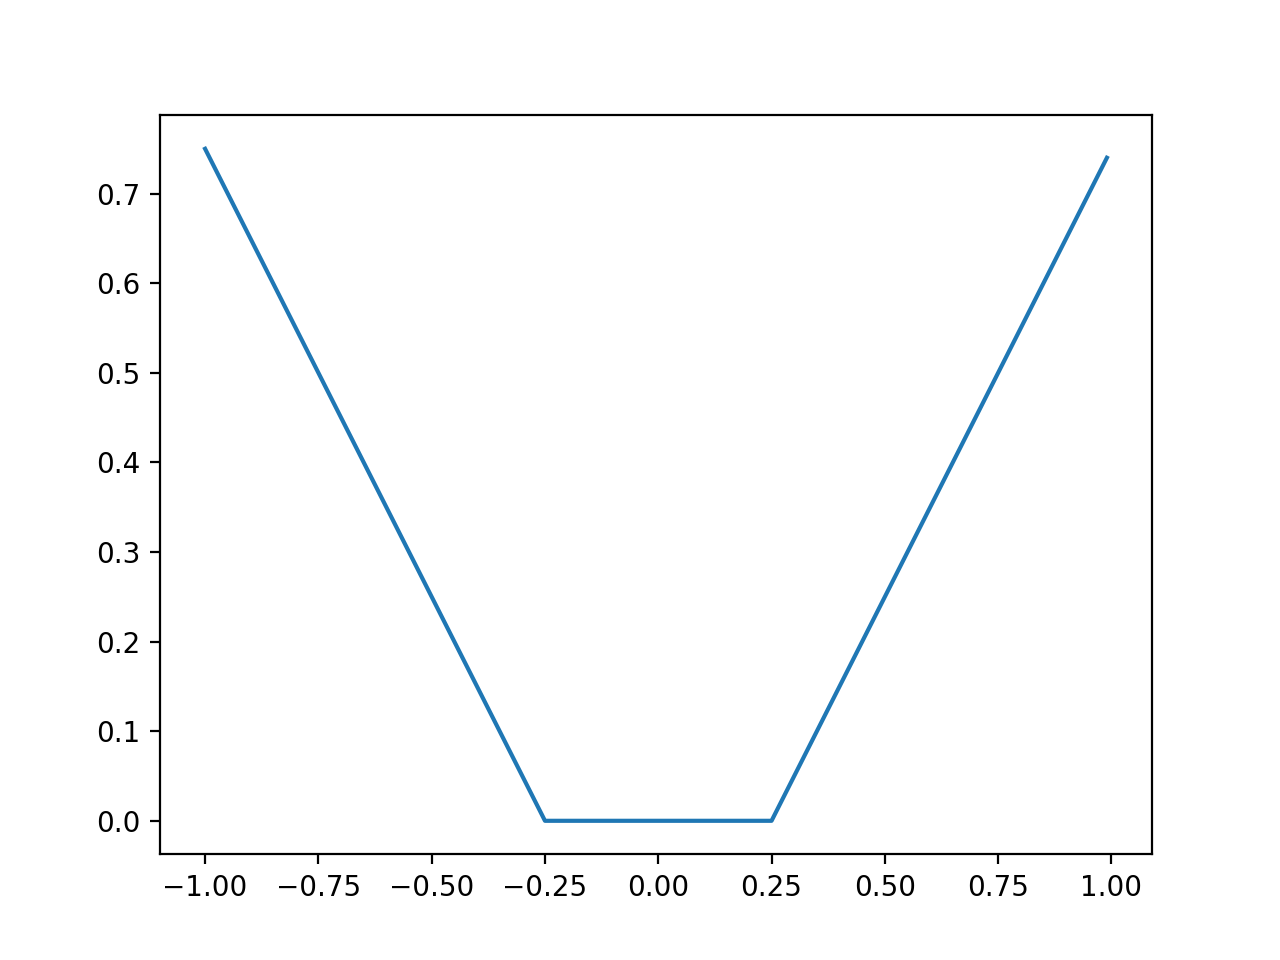
\includegraphics[width=0.6\textwidth]{Figures/SVM_loss.png}
\caption{\label{fig:SVM.V} The function $V$ defining the SVM risk function.}
\end{figure}

A plot of the function $V$ is provided in \cref{fig:SVM.V}. This function is an example of what is often called a robust
loss function. The quadratic error used in linear regression had the
advantage of providing closed form expressions for the solution, but is
quite sensitive to outliers. For robustness, it is preferable to use loss
functions that, like $V$, increase at most linearly at infinity. One sometimes  choose
them as smooth convex functions, for example $V(t) = (1-\cos\ga
t)/(1-\cos\ga\ep)$ for $|t|<\ep$ and $f(t) = |t|$ for $t \geq \ep$,
where $\ga$ is chosen so that $\ga\ep\sin\ga\ep /(1-\cos\ga\ep) =
1$. In such a case, minimizing
$$
F(\be) = \sum_{k=1}^N V(y_k - {a_0} - x_k^T b)
$$
can be done using gradient descent methods. Using  $V$ in \cref{eq:svm.v} will require a little more work, as we see now. 

The SVM regression problem is generally formulated as the minimization of
$$ 
\sum_{k=1}^N V(y_k - {a_0} - x_k^T b) + \la |b|^2\,,
$$
and we will study a slightly more general problem, minimizing
$$ 
F({a_0}, b) = \sum_{k=1}^N V(y_k - {a_0} - x_k^T b) + \la b^T \De b\,,
$$
where $\De$ is a symmetric positive-definite matrix.
This objective function exhibits the
following features:
\begin{enumerate}[label=$\bullet$,wide]
\item A penalty on the coefficients of $b$, similar to ridge regression.
\item A linear penalty (instead of quadratic) for large errors in the
prediction.
\item An $\ep$-tolerance for small errors, often referred to as {\em the margin} of the regression SVM.
\end{enumerate}

We now  describe the various steps in the analysis and reduction of
the problem. They will lead to simple minimization algorithms, and
possible extensions to nonlinear problems.



\paragraph{Reduction to a quadratic programming problem} 
Introduce  slack
variables $\xi_k, \xi_k^*, k=1, \ldots, N$. The original problem
is equivalent to the minimization, with respect to $({a_0}, b, \xi, \xi^*)$, of
$$
\sum_{k=1}^N (\xi_k+ \xi_k^*) + \la b^T\De b
$$
under the constraints:
\begin{equation}
\label{eq:svm.constr}
\left\{
\begin{aligned} 
&\xi_k, \xi_k^* \geq 0\\ 
&\xi_k - y_k + {a_0} + x_k^Tb +\ep \geq 0\\
&\xi_k^* + y_k - {a_0} - 
x_k^Tb +\ep \geq 0
\end{aligned}
\right.
\end{equation}
The simple proof of this equivalence, which results in a quadratic programming problem, is left to the reader. As often, one gains additional insight by studying the dual problem.



\paragraph{Dual problem}
Introduce $4N$ non-negative Lagrange multipliers for the  $4N$ constraints in the problem, namely,  $\eta_k, \eta_k^*\geq 0$ for the positivity constraints, and $\al_k,
\al_k^*\geq 0$ for the last two in \eqref{eq:svm.constr}. The resulting Lagrangian is
\begin{multline*}
\mathcal L ({a_0}, b , \xi, \xi^*, \alpha, \alpha^*, \eta, \eta^*) = \sum_{k=1}^N (\xi_k+ \xi_k^*) + \la b^T\De b - \sum_{k=1}^N
(\eta_k\xi_k + \eta_k^*\xi_k^*) \\
- \sum_{k=1}^N \al_k (\xi_k - y_k +
{a_0} + x_k^Tb + \ep)  - \sum_{k=1}^N \al_k^* (\xi^*_k + y_k - {a_0} -
x_k^Tb + \ep) .
\end{multline*}
In this formulation,
$({a_0}, b, \xi, \xi^*)$ are the primal variables, and $\alpha, \alpha^*,
\eta, \eta^*$ the dual variables.


The KKT conditions are provided by the system:
\begin{equation}
\label{eq:SVM.KKT}
\left\{\begin{aligned}
&\sum_{k=1}^N (\al_k-\al_k^*) = 0 \\
&2 \la \De b - \sum_{k=1}^N (\al_k-\al_k^*) x_k = 0\\
&1 - \eta_k - \al_k = 0 \\
&1 - \eta_k^* - \al_k^* = 0 \\
&\al_k (\ep + \xi_k - y_k + {a_0} +  x_k^Tb) = 0  \\
&\al_k^* (\ep + \xi_k^* + y_k - {a_0} - x_k^Tb) = 0  \\
&\eta_k\xi_k = \eta_k^*\xi_k^* = 0
       \end{aligned}
\right.
\end{equation}
The first four equations are the derivatives of the Lagrangian with respect to ${a_0}, b, \xi_k, \xi^*_k$ in this order and the last three are the complementary slackness conditions.

The dual problem maximizes the function 
$$
L^*(\al, \al^*, \eta, \eta^*) = \inf_{\be, \xi, \xi^*} \mathcal L.
$$
 under the previous
positivity constraints. 
Since the Lagrangian is linear in ${a_0}$,
$\xi_k$ and $\xi_k^*$, its minimum is $-\infty$ unless the
coefficients vanish. The linear terms must therefore vanish for $L^*$ to be finite. With these conditions plus the fact that  $\prt_b L = 0$, we retrieve the first four equations of system \eqref{eq:SVM.KKT}. 
Using $\eta_k  = 1- \al_k$, $\eta_k^* = 1- \al_k^*$ and 
\begin{equation}
\label{eq:svm.lin.b}
b = \frac1{2\la} \sum_{k=1}^N (\al_k-\al_k^*) \De^{-1} x_k
\end{equation}
one can 
express $L^*$ uniquely as a function of $\al, \al^*$, yielding
$$
L^*(\al, \al^*) = -\frac{1}{4\la} \sum_{k,l=1}^N
(\al_k-\al_k^*)(\al_l-\al_l^*) x_k^T\De^{-1} x_l - \ep \sum_{k=1}^N
(\al_k+\al_k^*) + \sum_{k=1}^N (\al_k-\al_k^*)y_k\,.
$$
This quantity must be maximized subject to the constraints  $0\leq \al_k,
\al_k^*\leq 1$ and $\sum_{k=1}^N (\al_k-\al_k^*) = 0$. This still is
a quadratic programming problem, but it now has nice additional features
and interpretations.


\paragraph{Step 3: Analysis of the dual problem}
The dual problem only depends on the $x_k$'s
through the matrix with coefficients $x_k^T\De^{-1} x_l$, which is the Gram matrix of $x_1, \ldots, x_N$ for the inner product associated with $\De^{-1}$. This property will lead to the the kernel version of SVMs discussed in the next section. The obtained predictor can
also be expressed as a function of these products, since
$$
y = {a_0} + x^T b = {a_0} + \frac{1}{2\la} \sum_{k=1}^N (\al_k-\al_k^*)
(x_k^T\De^{-1} x)\,.
$$
Moreover, the dimension of the dual problem is $2N$, which  allows the method to be used in large (possibly infinite) dimensions with a bounded cost.

%The parameter ${a_0}$ can be determined  using the KKT conditions when the optimal $\al, \al^*$ are computed. 
We now analyze the solutions   $\al, \al^*$ of the dual problem. The complementary slackness conditions reduce to:
\begin{equation}
\label{eq:SVM.slackness}
\left\{\begin{aligned}
&\al_k (\ep + \xi_k - y_k + {a_0} + x_k^T b) = 0  \\
&\al_k^* (\ep + \xi_k^* + y_k - {a_0} - x_k^T b) = 0  \\
&(1-\al_k)\xi_k = (1-\al_k^*)\xi_k^* = 0
\end{aligned}
\right.
\end{equation}
These conditions have the following consequences,  based on the prediction error made for each training sample.
\begin{enumerate}[label=(\roman*), wide=0.5cm]
\item First consider indexes $k$
such that the error is strictly within the tolerance
margin $\epsilon$: $|y_k - {a_0} - x_k^Tb| < \ep$. Then the terms between parentheses in first two equations of \eqref{eq:SVM.slackness} are strictly positive, which implies that $\al_k = \al_k^* = 0$. The last two equations in \eqref{eq:SVM.slackness} then imply $\xi_k  = \xi_k^* = 0$. 
\item Consider now the case when the prediction is strictly less accurate
than the tolerance margin. Assume that $y_k - {a_0} - x_k^Tb > \ep$. The second and third equations in \eqref{eq:SVM.slackness} imply that $\al_k^* = \xi_k^* = 0$. The assumption also implies that 
\[
\xi_k = y_k - {a_0} - x_k^Tb -\ep >0
\]
and $\al_k = 1$. The case $y_k - {a_0} - x_k^Tb < - \ep$ is symmetric and provides $\al_k = \xi_k = 0$, $\xi_k^*  >0$
and $\al_k^* = 1$.

\item Finally, consider samples for which the prediction error is exactly
at the tolerance margin. If $y_k - {a_0} - x_k^T b = \ep$, we have $\al_k^* = \xi_k = \xi_k^* =0$. The fact that $\al_k^* = \xi_k^*=0$ is clear. To prove that $\xi_k=0$, we note that would have otherwise  $\xi_k - y_k + {a_0} + x_k^Tb +\ep > 0$, which would imply that $\al_k=0$ and we  reach a contradiction with $(1-\al_k)\xi_k=0$. Similarly, $y_k - {a_0} - x_k^T b = -\ep$ implies that $\al_k = \xi_k = \xi_k^* =0$.

The points for which $|y_k - {a_0} - x_k^T b| = \ep$ are called {\em support vectors}.
\end{enumerate}

One important information deriving from this discussion is that the variables $(\al_k, \al_k^*)$ have prescribed values as long as the error $y_k - {a_0} - x_k^T b$ is not exactly $\ep$ in absolute value: $(1,0)$ if the error is larger than $\ep$, $(0,0)$ if it is strictly between $-\ep$ and $\ep$ and $(0,1)$ if it is less than $-\ep$. Also in all cases, at least one of $\al_k$ and $\al_k^*$ must vanish. Only in the case of support vectors does the previous discussion fail to provide a value for one of these variables.

Now, we want to reverse the discussion and assume that the dual problem is solved to see how the variables ${a_0}$ and $b$ of the primal problem can be retrieved. For $b$, this is easy, thanks to \eqref{eq:svm.lin.b}. For ${a_0}$ a direct computation can be made if a support vector is identified, either because $0 < \al_k <1$, which implies that ${a_0} = y_k - x_k^Tb -\ep$, or because 
$0 < \al^*_k <1$, which yields ${a_0} = y_k - x_k^Tb +\ep$.

If no support vector can be identified, ${a_0}$ is not uniquely determined (note that the objective function is not strictly convex in ${a_0}$). However, the coefficients $\al_k, \al_k^*$ provide some information on this intercept, in the form of inequalities. More precisely, let
$J^+ =  \{k : \al_k = 1\}$, $J^- = \{k:\al_k^* = 1\}$ and $J_0 = \{k:\al_k = \al_k^* = 0\}$. Then $k \in J^+$ implies that 
$y_k - {a_0} - b^Tx_k \geq \ep$, so that ${a_0} \leq y_k - b^T x_k -\ep$. Similarly, $k\in J^-$ implies that ${a_0} \geq y_k - b^T x_k +\ep$. Finally, $k\in J_0$ implies that ${a_0} \geq y_k - b^T x_k -\ep$ and ${a_0} \leq y_k - b^T x_k +\ep$. As a consequence, one can take ${a_0}$ to be any point in the interval $[{a_0}^-, {a_0}^+]$, where
\begin{align*}
{a_0}^- &= \max\left(\max_{k\in J^-} (y_k - x_k^Tb + \ep), \max_{k\in J_0} (y_k - x_k^T b - \ep)\right)\\
{a_0}^+ &= \min\left(\min_{k\in J^+} (y_k - x_k^Tb - \ep), \min_{k\in J_0} (y_k - x_k^T b + \ep)\right).
\end{align*}
%
%
%
%${a_0}$ can be any value satisfying
%\[
%\left\{
%\begin{aligned}
%&\max_{k\in J^-} (y_k - x_k^Tb + \ep) \leq {a_0} \leq \min_{k\in J^+} (y_k - x_k^Tb - \ep)\\
%&\max_{k\in J_0} (y_k - x_k^T b - \ep) \leq {a_0} \leq \min_{k\in J_0} (y_k - x_k^T b + \ep)
%\end{aligned}
%\right.
%\]
%(with $x_k^Tb = \sum_{l=1}^N (\al_k-\al_k^*) (x_k^Tx_l)/(2\la)$).
%
%Note also that $\al_k$ and $\al_k^*$ cannot be nonzero together
%(because they correspond to incompatible constraints), and that when
%they are both zero, the corresponding points do not contribute to the
%estimation. Finally, for all points except support vectors, their value is either 0 or 1. 


\subsection{The kernel trick and SVMs}
Returning to our feature space notation, let $X$ take values in $\CR_X$ and $h: \CR_X \to H$ be a feature function with values in an inner-product space $H$ with associated kernel $K$. SVMs in feature space must minimize, with ${a_0}\in \mR$ and $b\in H$
$$ 
F({a_0}, b) = \sum_{k=1}^N V\big(y_k - {a_0} - \scp{h(x_k)}{b}_H\big) + \la \|b\|_H^2\,.
$$
Letting as before $V = \vspan(h(x_1), \ldots, h(x_N))$, the same argument as that made for ridge regression works, namely that the first term in $F$ is unchanged if $b$ is replaced by $\pi_V(b)$ and the second one is strictly reduced unless $b\in V$, leading to a finite-dimensional formulation in which 
\[
b = \sum_{k=1}^N c_k h(x_k)
\]
and one minimizes
$$ 
F({a_0}, c) = \sum_{k=1}^N V\Big(y_k - {a_0} - \sum_{l=1}^N K(x_k,x_l) c_l\Big) + \la \sum_{k,l=1}^N K(x_k,x_l) c_kc_l \,.
$$
This function has the same form as the one studied in the linear case with $b$ replaced by $c \in \mR^N$, $x_k$ replaced by the vector with coefficients $K(x_k, x_l), l=1, \ldots, N$, that we will denote $\CK^{(k)}$ and $\De = \CK = \CK(x_1, \ldots, x_N)$. Note that $\CK^{(k)}$ is the $k$th column of $\CK$, so that 
\[
\big(\CK^{(k)}\big)^T \CK^{-1} \CK^{(l)} = K(x_k, x_l).
\]
Using this, we find that the dual problem requires  to maximize
$$
L^*(\al, \al^*) = -\frac{1}{4\la} \sum_{k,l=1}^N
(\al_k-\al_k^*)(\al_l-\al_l^*) K(x_k, x_l) - \ep \sum_{k=1}^N
(\al_k+\al_k^*) + \sum_{k=1}^N (\al_k-\al_k^*)y_k\,.
$$
with
$$
\left\{
\begin{aligned}
&0\leq \al_k \leq 1 \\
&0 \leq  \al_k^* \leq 1 \\
&\sum_{k=1}^N (\al_k-\al_k^*) = 0 \\
\end{aligned}
\right.
$$
The associated vector $c$ satisfies
\[
2 \la c =  \sum_{k=1}^N (\al_k-\al_k^*) \CK^{-1} \CK^{(k)} = \al - \al^*\,.
\]
and the regression function is
\[
f(x) = {a_0} + \scp{b}{h(x)}_H = {a_0} + \frac{1}{2\la} \sum_{k=1}^N (\al_k-\al_k^*)  K(x, x_k)\,.
\]
Finally, the discussions on the values of $\al, \al^*$ and on the computation of ${a_0}$ remain unchanged.





%\subsection{Extension to other loss functions}
%This $\ep$-tolerant function is the most commonly used loss function
%in the SVM literature. However, the previous analysis would not be much
%affected if $V(t)$ were replaced by some other function $C(t) =
%c_0(t-\ep)$ if $t\geq \ep$ and 0 otherwise, with a convex
%$c_0$. In  the linear case,  the primal problem becomes: minimize
%$$
%{\la} |b|^2 + \sum_{i=1}^N (c_0(\xi_k) + c_0(\xi_k^*))
%$$
%with the constraints 
%$$
%-\ep - \xi_k^* \leq y_k - {a_0} - x_k\be \leq \ep+\xi_k
%$$
%and $\xi_k, \xi_k^* \geq 0$. This is a convex programming problem. Its
%equivalent dual formulation is: maximize
%\begin{multline*}
%- {\la} \sum_{k,l=1}^N (\al_k-\al_k^*) (x_k^Tx_l)
%(\al_l-\al_l^*) + \sum_{k=1}^N (\al_k-\al_k^*)y_k - \ep \sum_{i=1}^N
%(\al_k+\al_k^*) \\+  \sum_{k=1}^N (T(\xi_k) + T(\xi_k^*))
%\end{multline*}
%with the constraints $\al_k, \al_k^*\xi_k, \xi_k^* \geq 0$, $\sum_k (\al_k-\al_k^*)
%= 0$, $\xi_k = \inf\defset{t, c'_0(t) > \al}$, and the notation
%$$
%T(u) = c_0(u) - u c'_0(u).
%$$
%The dual formulation still has the property to depend only on the
%inner products $x_k^Tx_l$, so that a kernel extension is still valid.
%






